\chapter{Applications}

In this chapter, we provide examples of some typical results which can be obtained with OSCAR. These examples could be taken as a starting point to build more complex simulations. The OSCAR scripts associated with each examples are provided in the OSCAR package. The example described here are using the classic version of OSCAR (version 1.X) which can be downloaded here \cite{OS_down}.\textbf{ For new user, it is recommended to use OSCAR V3.x and so jump directly to the section \ref{ch4:ex}}

\section{Distortion of the optical field due to thermal lensing}\label{cha3.1}

Let's consider the same Fabry-Perot cavity as the one described in the previous chapter (section \ref{chap2:1}). Instead of using an input laser beam of 1~W, we upgrade the input power to 500~W (so the circulating power is now 375~kW) and we are interested to simulate some thermal lensing. Both input and end mirrors are supposed to be made of fused silica with a substrate absorption of 2~ppm/cm and a coating absorption of 0.5~ppm.

At least two distinctive effects can be induced due to the optical power absorbed in the mirrors:
\begin{itemize}
  \item A temperature gradient inside the substrates of the mirrors appears. The temperature gradient generates a refractive index gradient (thermo-optic effect) which induces a wavefront distortion for the beam crossing the optics.
  \item Since the temperature is no longer uniform in the test mass, the curvature of the optic surface will change as a result of thermal expansion. In this case we can expect the eigen mode of the cavity to change as well.
\end{itemize}

Before we continue, it is better to make some assumptions to lighten the calculations. If the reader understands the method described here it is straight forward to implement a full model. First we will suppose that we have uniform absorption in the test mass, so we can take advantage of the cylindrical symmetry. The power absorbed is dominated by the coating absorption, so we will only take into account the temperature gradient $T(r,z)$ in the optics and the thermal expansion of the mirror high reflective (HR) coating surface $\delta s(r)$. The deformations of the anti reflective coating are assumed to be negligible.

OSCAR can not simulate directly the effect of the optical absorption. If required an analytical formula can be implemented \cite{Hello321} however it is not as flexible as finite element simulations in particular if thermal lensing compensation scheme has to be investigated. I used the software ANSYS to simulate the temperature gradient $T(r,z)$ in the optics and the thermal expansion of the mirror surface $\delta s(r)$\footnote{We assume uniform absorption in the test mass, so we can take advantage of the cylindrical symmetry.}. A schematic of the hot cavity is shown in figure \ref{fig3:hotcav}.

\begin{figure}
\begin{center}
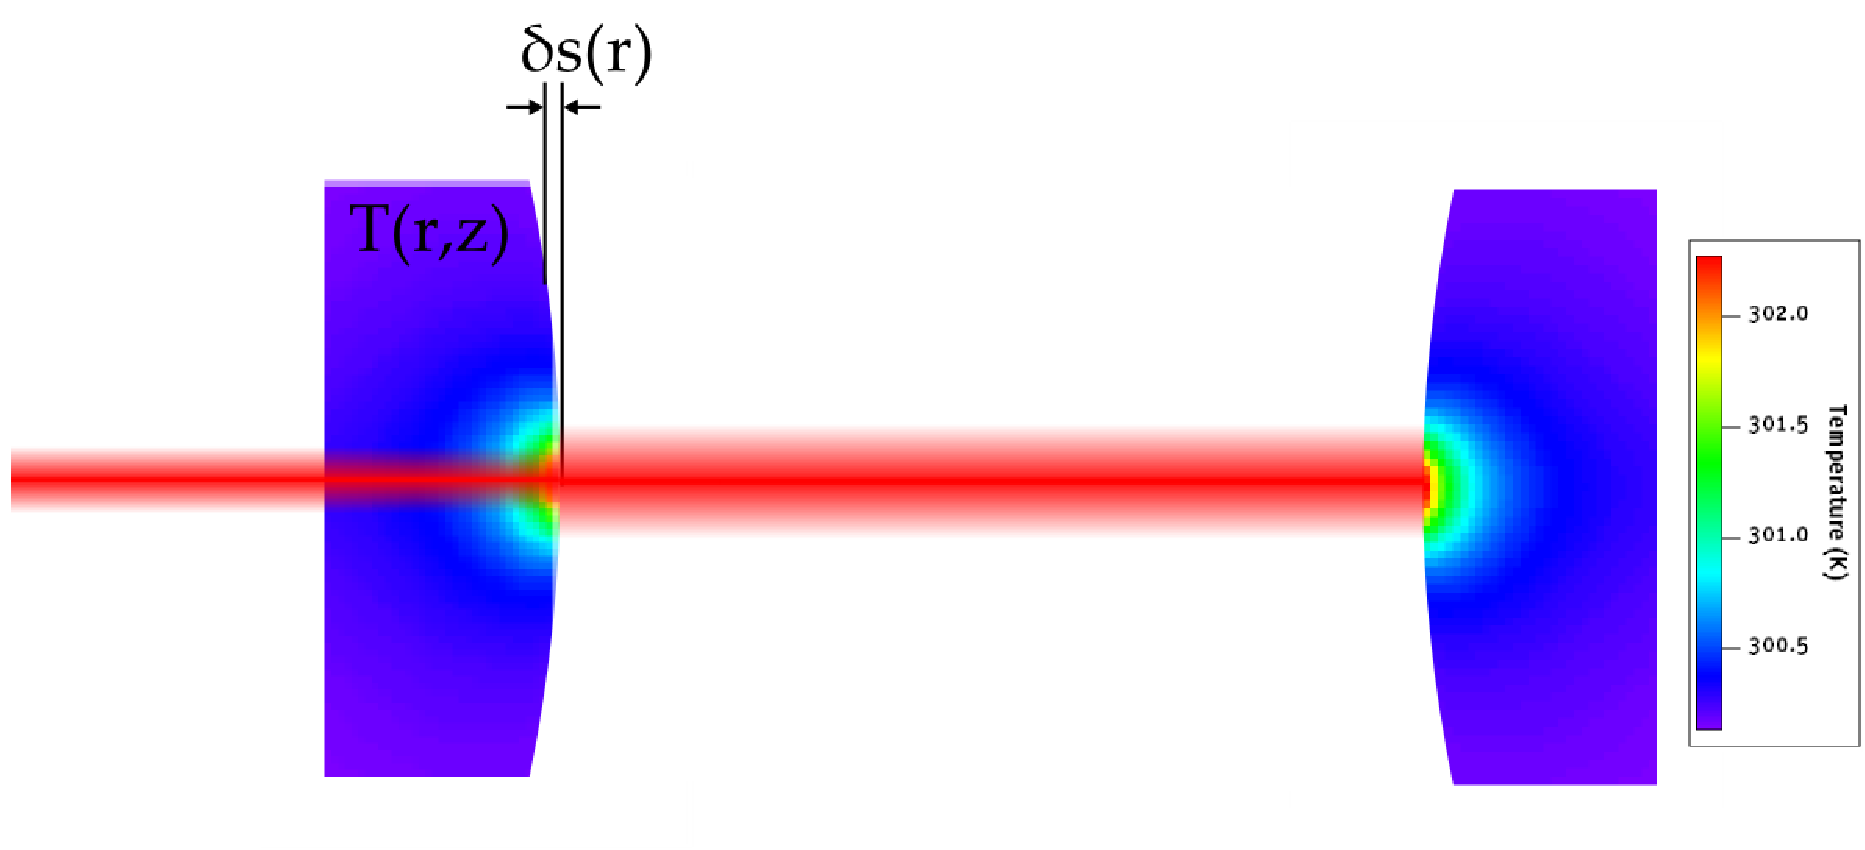
\includegraphics[width = 0.95\textwidth]{Fig3_Hot_cav2.pdf}
\end{center}
\caption{\label{fig3:hotcav} Schematics of the hot cavity. The mirror diameter is 250~mm and the thickness is 100~mm. We can notice that the temperature profile is dominated by the coating absorption. The optical parameters are detailed in the text. For clarity, we did not represent the curvature of the cold optics and we suppose the same distortion in the input and end mirrors. $T(r,z)$ represents the temperature distribution inside the test mass and $\delta s(r)$ the change in sagitta due to the optical absorption.}
\end{figure}

From the temperature distribution inside the substrate and the sagitta change, we can derive the optical path length difference $\Delta OPN_{sub}^{trans}(r)$ induced by the substrate in transmission according to:

\begin{eqnarray}\label{eq3:OPN1}
  \Delta OPN_{sub}^{trans}(r) &=& \int_0^L n(r,z) dz - \int_0^L n(0,z) dz + (n-1)\delta s(r) \nonumber \\
                &=&  \int_0^L \beta T(r,z) dz - \int_0^L \beta T(0,z) + (n-1)\delta s(r) dz
\end{eqnarray}

With $\beta$ the thermo-optic coefficent and n the refractive index of the substrate. Similarly, we can calculate the wavefront distortion $\Delta OPN_{sub}^{ref}(r)$ for the input beam reflected directly reflected on the input mirror:

\begin{equation}\label{eq3:OPN2}
  \Delta OPN_{sub}^{ref}(r) = 2\left( \int_0^L \beta T(r,z) dz - \int_0^L \beta T(0,z) + n\delta s(r) \right)
\end{equation}

And finally, the wavefront distortion of the beam reflected on the mirrors inside the cavity is:

\begin{equation}\label{eq3:OPN3}
  \Delta OPN_{cav}^{ref}(r) = 2 \delta s(r)
\end{equation}

Of course, the three wavefront distortions just defined, have to be added to any wavefront distortion already present when the cavity is cold, especially the ones induced by the curvature of the mirrors. For references, the main distortions due to thermal lensing which have to be included in OSCAR are plotted in figure \ref{fig3:OPN}.\\

Here an example how to proceed in reality. First run ANSYS to simulate the temperature distribution in the test mass as well as the thermal expansion of the optic. Then from these results, we can save a text file with two results, first the wavefront distortion induced by the thermo-optic effect for the optic in transmission and the change in sagitta of the optics. The text file is then loaded in OSCAR and the new wavefront distortions for the all optics of the cavity are calculated accordingly. An example of such a text file is presented below, the first column is the radius, the second the optical path length difference in transmission and the third the change in sagitta, all the columns are in meter.

\begin{verbatim}
 -1.2500000e-001 -1.0824598e-006 -2.6695000e-008
 -1.2142857e-001 -1.0731224e-006 -2.6433549e-008
 -1.1785714e-001 -1.0655394e-006 -2.6172131e-008
 -1.1428571e-001 -1.0577238e-006 -2.5911061e-008
 -1.1071429e-001 -1.0496365e-006 -2.5695000e-008
 -1.0714286e-001 -1.0398661e-006 -2.5695000e-008
 -1.0357143e-001 -1.0304229e-006 -2.5615955e-008
 -1.0000000e-001 -1.0216618e-006 -2.5349271e-008
\end{verbatim}

The file can found in the OSCAR distribution under the name \textcolor{blue}{From\_ANSYS.txt} in the folder \textcolor{blue}{Calculate\_TL\_effect}. A graphical representation of the data file from ANSYS is shown in figure \ref{fig3:OPN}.

% 17*11 cm

\begin{figure}
\begin{center}
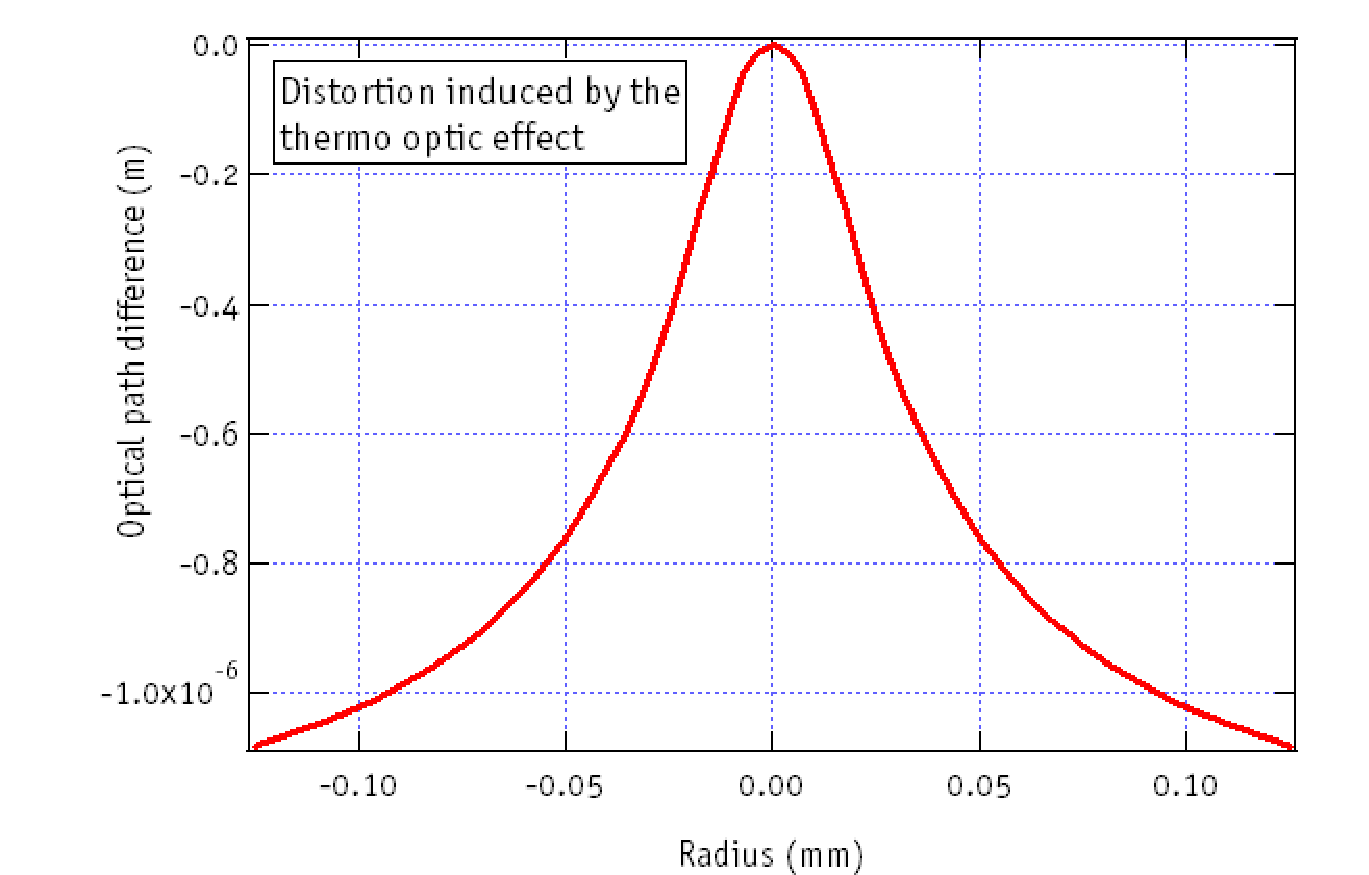
\includegraphics[width = 0.50\textwidth]{Fig3_OPN1.pdf}\hfill
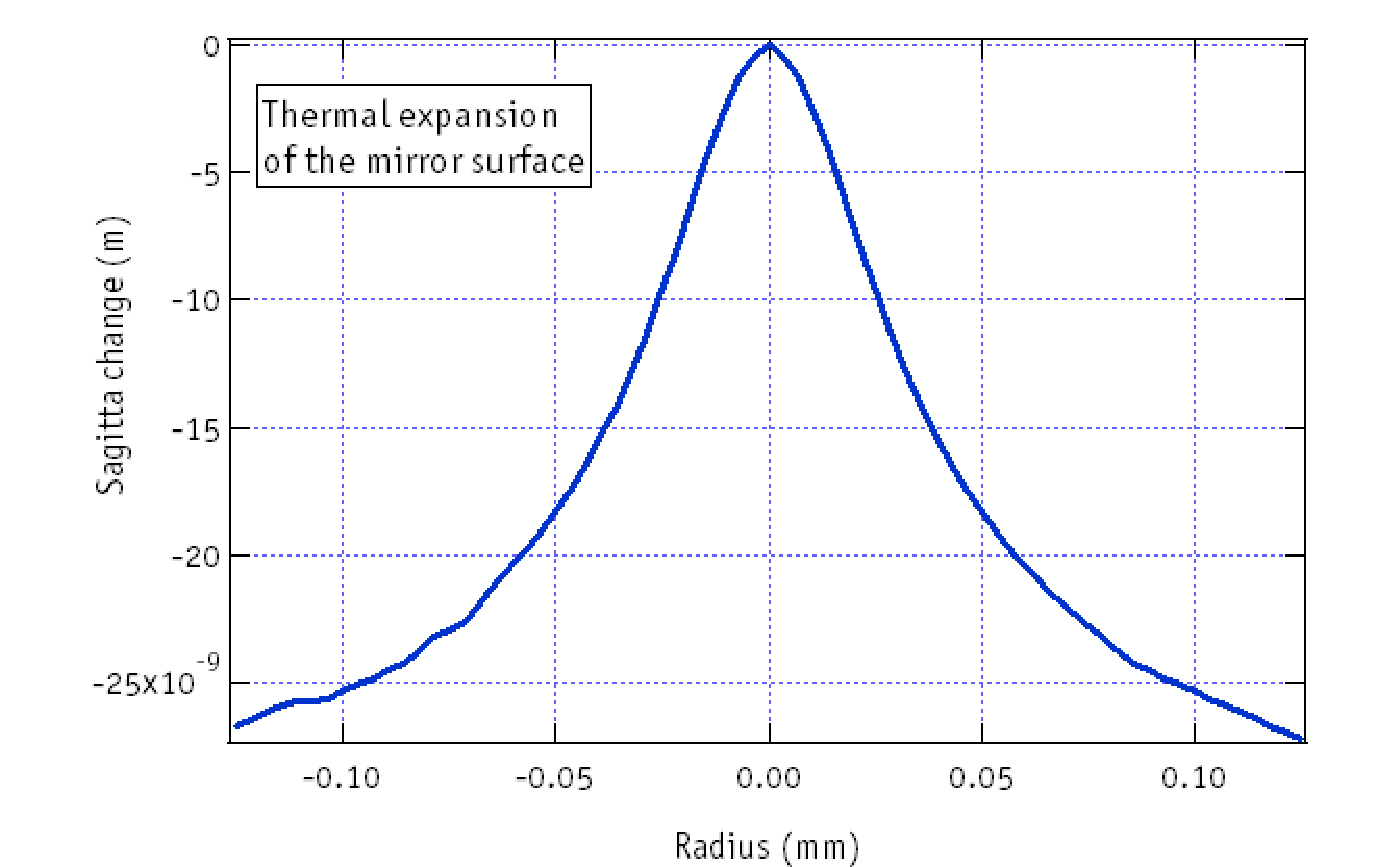
\includegraphics[width = 0.50\textwidth]{Fig3_OPN2.pdf}
\end{center}
\caption{\label{fig3:OPN} Optical path length difference induced by the mirror substrates in transmission when only the thermo optics effect is considered (left) and change in the sagitta of the reflective side of the mirrors (right). It interesting to note the difference between the two vertical scales, the left plot represents an optical path in micrometers, whereas the right plot is in tens of nanometers. These plots are derived from the results of ANSYS simulations and will then be integrated into OSCAR.}
\end{figure}

Most of the time, the resolution used with the results file from ANSYS is different from the grid resolution used in OSCAR so we have to resample the results using an interpolation method. How the results file is integrated into OSCAR is presented into the listing \ref{lis3:read}

\begin{lstlisting}[float=tp,caption=Commands used to read thermal lensing results from ANSYS. \label{lis3:read},frame=lines]
% Load the results file
load('From_ANSYS.txt')
loaded.radius = From_ANSYS(:,1);
loaded.TL = interp1(From_ANSYS(:,1),From_ANSYS(:,2),Grid.D2,'spline')*0.2;
loaded.sag = interp1(From_ANSYS(:,1),From_ANSYS(:,3),Grid.D2,'spline')*0;

% Add the thermal lensing distortion to the previous wavefront
% Special attention to the sign!

Mirror.ITM_cav = Mirror.ITM_cav - 2*loaded.sag;
Mirror.ETM_cav = Mirror.ETM_cav - 2*loaded.sag;

Mirror.ETM_trans = Mirror.ETM_trans + loaded.TL - (Refrac_index-1)*loaded.sag;
Mirror.ITM_trans = Mirror.ITM_trans + loaded.TL - (Refrac_index-1)*loaded.sag;

Mirror.ITM_ref = Mirror.ITM_ref + 2*loaded.TL - 2*Refrac_index*loaded.sag;
\end{lstlisting}

After implementing the distorted mirrors, we can calculate the resonance length for the fundamental mode and then calculate the total circulating field. This is done by running successively the scripts \textcolor{blue}{Find\_resonance\_length.m} and \textcolor{blue}{Get\_results.m}. The comparison between the cold cavity is presented in table \ref{tab3:res}.

\begin{table}[tbp]
  \centering
  \caption{\label{tab3:res} Comparison of the cavity gain and size of the beam on the input mirror for a cavity with and without thermal lensing.}
\begin{tabular}{|l |c|c|}
\hline
{\large\strut} & Cold cavity & Hot cavity \\
\hline
{\large\strut} Cavity gain & 749.3 & 444.8 \\
{\large\strut} Beam radius on IM (mm)& 20.6 & 20.8 \\
\hline
\end{tabular}
\end{table}

Some very interesting points can be deduced by understanding the two lines of the table \ref{tab3:res}:

\begin{itemize}
  \item Due to thermal lensing, the beam radius only increases by 1~\%. That indicates that the mirror profiles are only slightly affected by thermal lensing since the cavity eigen modes are very similar for both cases: cold and hot cavities. This is not a surprise since the change in sagitta of the reflective sides of the mirrors is relatively small as we have previously seen.
  \item The decrease in the optical gain is quite important, since the optical gain is almost divided by a factor 2 between the cold and hot cases. It means in the hot cavity case, we have a strong mode mismatching between the input beam and the cavity fundamental mode. Since the latter has almost not changed, we can deduce that the mode mismatching is induced by the thermal lens in the substrate of the input mirror.
  \item We have assumed a certain amount of optical power absorbed in the mirror, it was based on the optical power circulating in the cold cavity. But since the circulating has decreased due to the mode mismatching, our thermal lens calculating wrong. A simple iterative process can be written to solve this problem and find the steady state parameters.
  \item This simple example shows that in our fused silica mirrors, the main thermal lensing effect is due to the thermal lens in the substrate of the input mirror generated by the optical absorption in the high reflective coating. The conclusion may be different for different substrates such as sapphire or calcium fluoride.
\end{itemize}

\section{Calculating diffraction losses}
\label{cha3.2}

One of the most promising application of FFT optical codes is to calculate the diffraction loss of the circulating cavity field. The method used to calculate the diffraction loss has been explained in section \ref{sec2:6}. An example how to calculate the diffraction loss of the mode HG$_{10}$ is presented in the folder \textcolor{blue}{Calculate\_diffraction\_loss}.

The diffraction loss calculation can be decomposed into three steps:
\begin{enumerate}
  \item Find the resonance length of the cavity for the mode HG$_{10}$. For that we can inject a mode HG$_{10}$ and maximise the circulating power. This approach is too easy, instead we will inject a uniform pattern of light and excite all the optical modes HG$_{m0}$. Then we will select manually the resonance length of the mode HG$_{10}$ in the spectrum of the cavity.
  \item Find the HG$_{10}$ eigen mode of the cavity. The shape of this mode can be different from the theory if the mode undergoes some serious clipping.
  \item Calculate the diffraction loss as the power lost during one light round trip with perfect reflective mirror.
\end{enumerate}

We decide to not inject directly a mode HG$_{10}$ (right plot on figure \ref{fig3:strip}) but instead inject a simpler light pattern which will excite all the optical modes along the horizontal axis. This pattern is one vertical strip with positive amplitude and one vertical strip with negative amplitude as shown in the left plot figure \ref{fig3:strip}.\\

\begin{figure}
\begin{center}
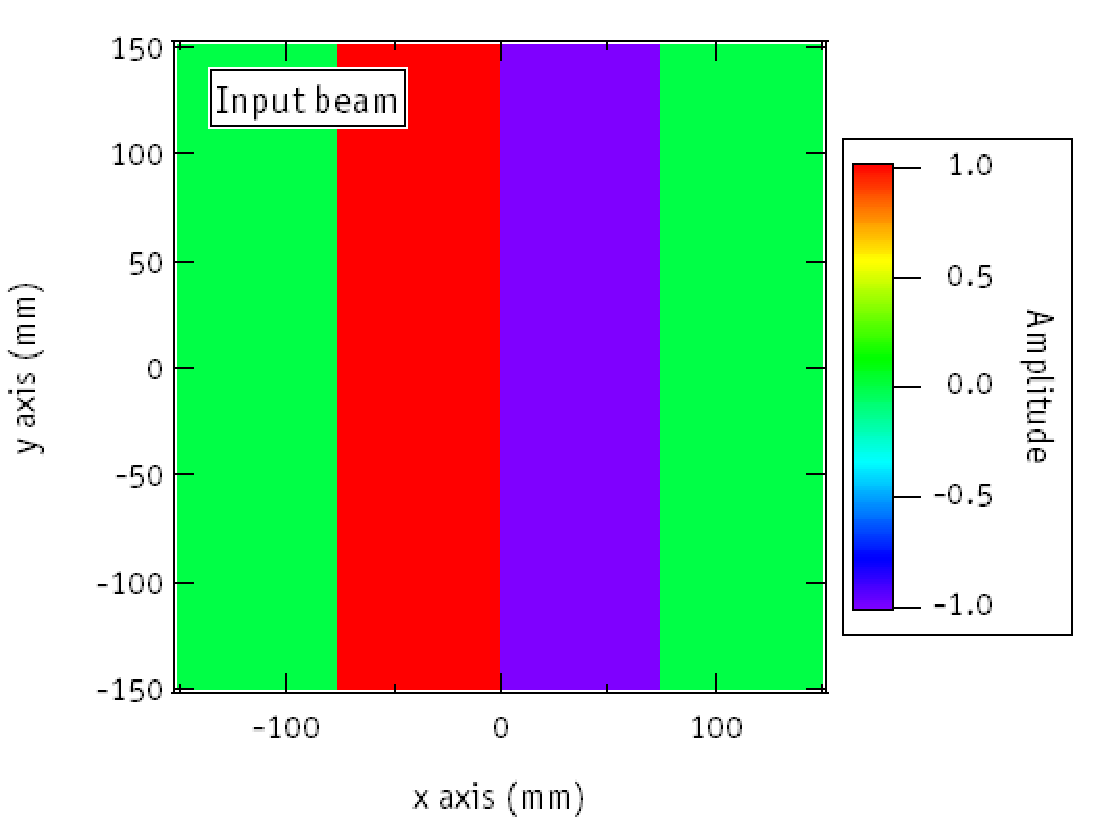
\includegraphics[width = 0.50\textwidth]{Fig3_inputbeam.pdf}\hfill
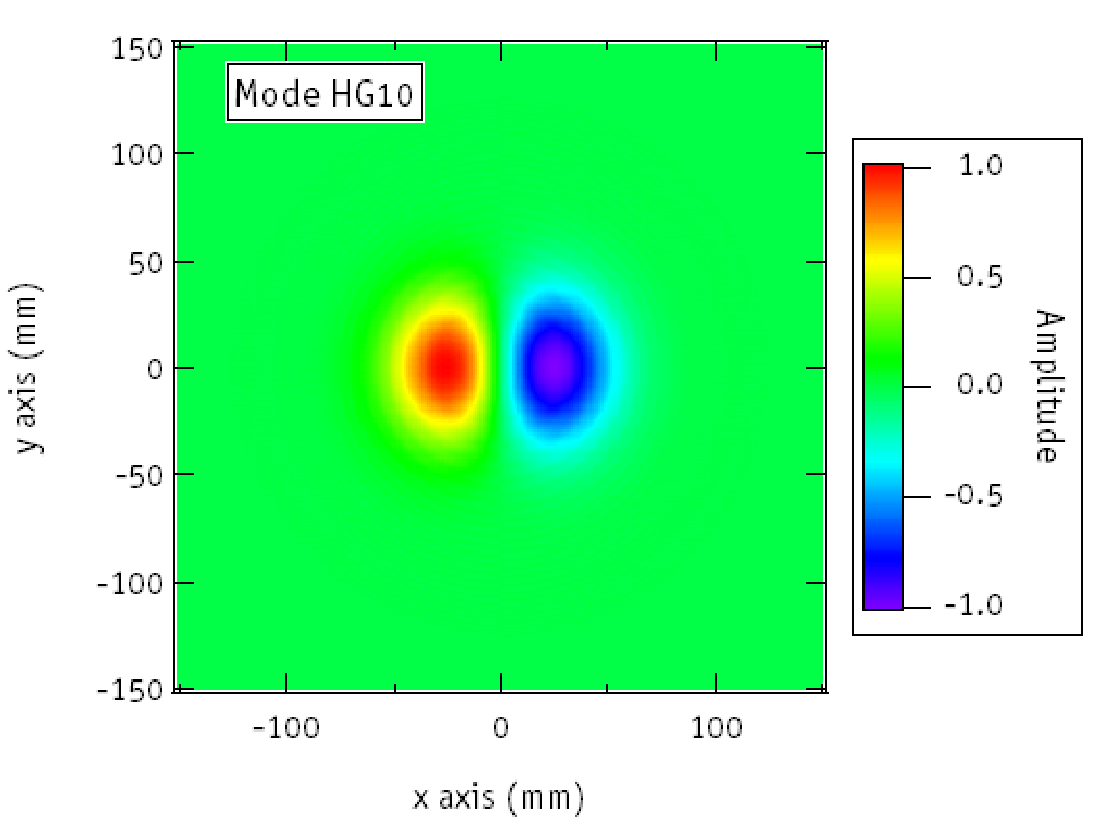
\includegraphics[width = 0.50\textwidth]{Fig3_HG10.pdf}
\end{center}
\caption{In the left plot, is the profile of the input electric field that we inject in the cavity to excite the HG$_{10}$ shown on the right. Both optical pattern are normalised in amplitude.\label{fig3:strip}}
\end{figure}

By using the procedure \textcolor{blue}{Find\_resonance\_length.m}, we can calculate all the cavity modes excited due to our particular input beam. The circulating power as the cavity is scanned over one FSR is shown in figure \ref{fig3:cav_spec}. Each peak in this plot represents the resonance of one of the cavity mode. We can display different cavity eigen modes for the first four highest peaks and we found that the mode HG$_{10}$ resonates for a detuning of $3.181\times 10^{-7}$~m.

\begin{figure}
\begin{center}
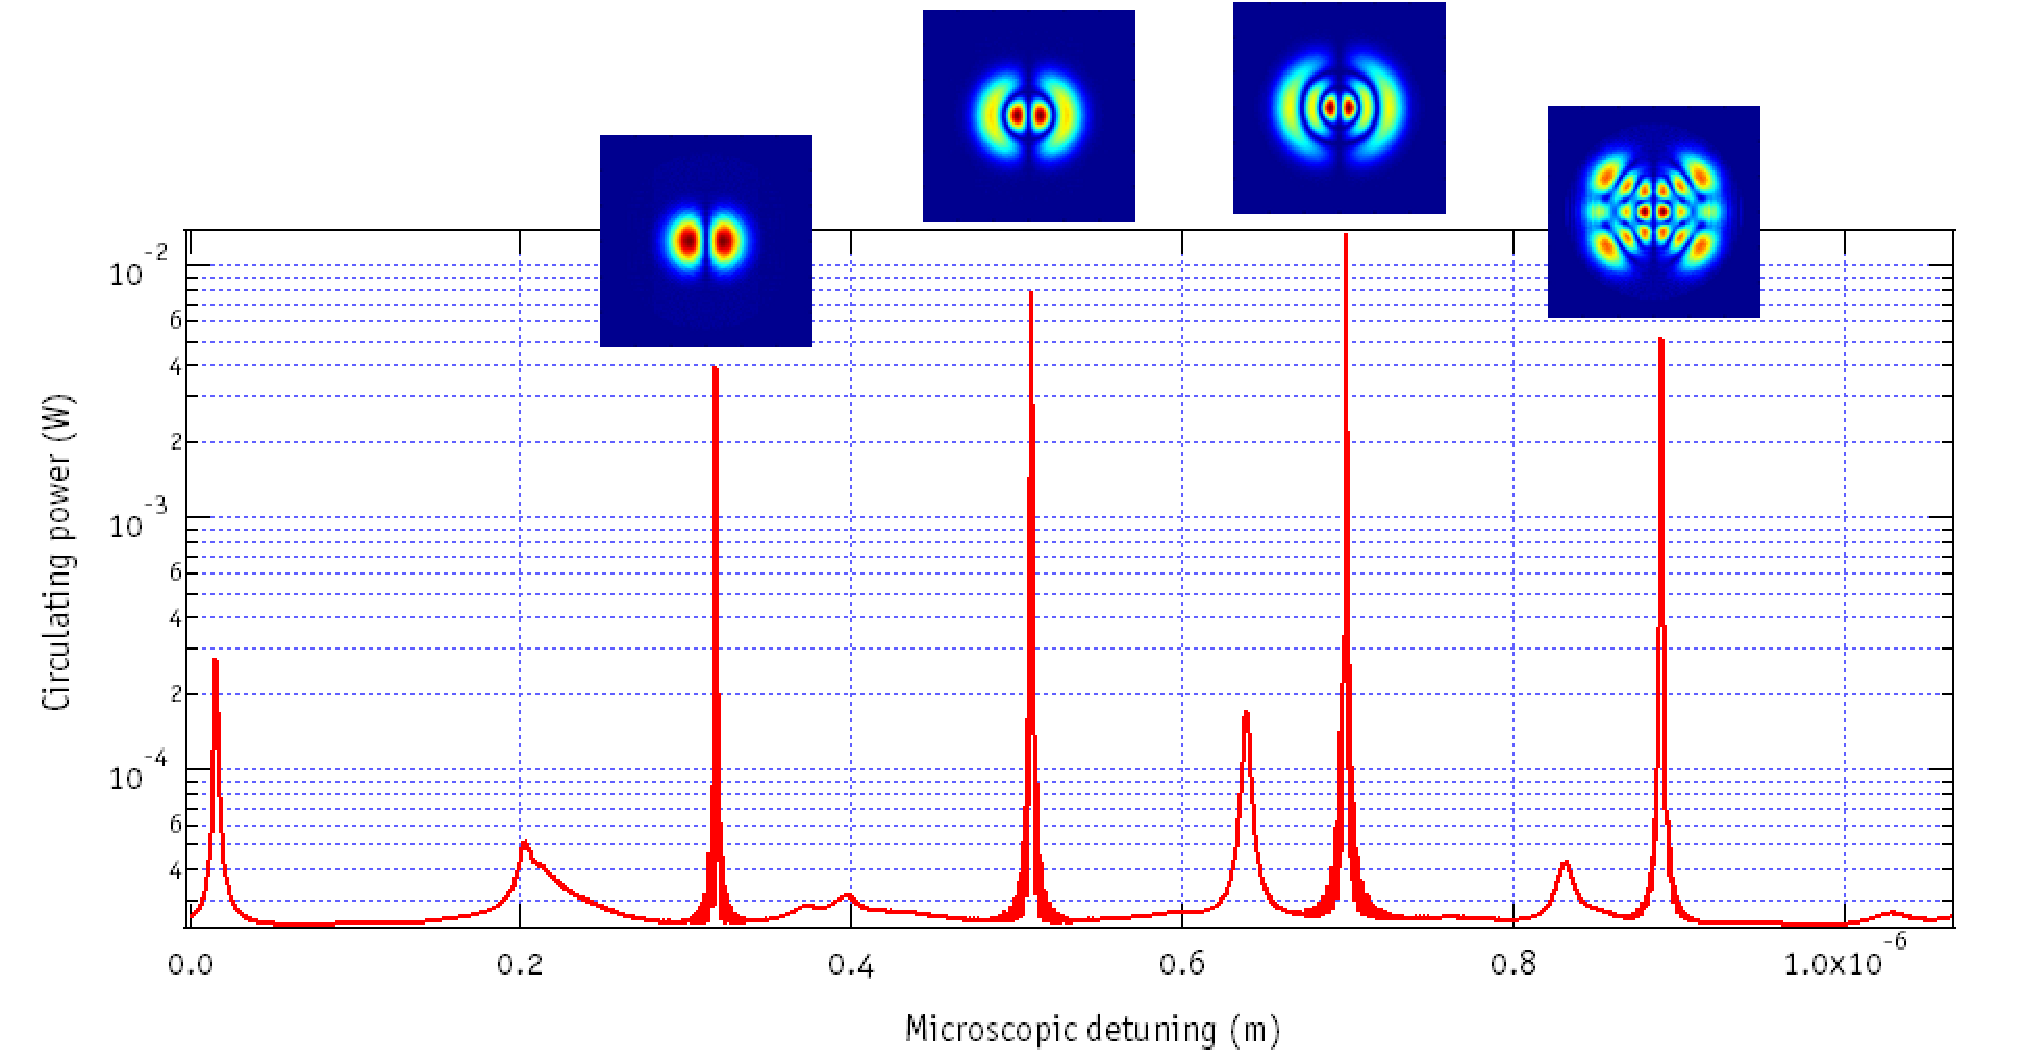
\includegraphics[width = 1\textwidth]{Fig3_Spectrum.pdf}
\end{center}
\caption{Cavity spectrum showing the different resonance lengths of the optical modes. The power profile of the main optical modes is presented above their respective resonance peaks.\label{fig3:cav_spec}}
\end{figure}

Since we have found the resonance length for the mode HG$_{10}$, we can now use the procedure \textcolor{blue}{Get\_results.m} to calculate the diffraction loss using the method described in section \ref{sec2:6}. As the result we found the diffraction loss equal to 618 ppm per round trip. Important beam clipping can also change the shape of the eigen mode of the cavity, this can be easily demonstrated using a FFT code\cite{Pab}.

We can now check how the diffraction loss depends of the size of the grid. The results are shown in \ref{tab3:grid_size}. As we can see the results do not change as we increase the size of the grid (which is a good sign). Below a grid size of 128 $\times$ 128, no realistic eigen modes can be found in the cavity.

\begin{table}[tbp]
  \centering
  \caption{\label{tab3:grid_size} Influence of the size of the grid on the diffraction loss).}
\begin{tabular}{|l|c|}
\hline
{\large\strut} Size of the grid  & Diffraction loss (ppm) \\
\hline
{\large\strut} 128 $\times$ 128 &  618 \\
{\large\strut} 256 $\times$ 256 &  620 \\
{\large\strut} 512 $\times$ 512 &  621 \\
\hline
\end{tabular}
\end{table}



\section{Using flat beams}
\label{cha3.3}

In this section, we will show how OSCAR can be used to calculate the frequency separation between higher order modes. This is in fact an indirect calculation of the Gouy phase shift between optical modes. To make the example more interesting, we will not use the usual Gaussian beams but flat beams. As a consequence of using flat beams, the mirrors of our cavity will no longer have spherical profiles \cite{Flat}.\\

To create the mirror profiles, we will not use directly the analytical formula which is relatively complicated, but instead we will use the wavefront curvature of the flat beam at the mirror position. Since the flat beam is an eigen mode of the cavity, the curvature of the mirrors must match the wavefront of the incoming beam. So the three steps to calculate will be:

%http://scitation.aip.org/getabs/servlet/GetabsServlet?prog=normal&id=PRVDAQ000074000008082002000001&idtype=cvips&gifs=yes


\begin{enumerate}
  \item Use the simple analytical formula to define the flat beam at the waist of the cavity. Since both mirror will have identical profile, we know that the waist position is in the middle of the cavity.
  \item Propagate the beam along half the cavity length, so the flat beam is now at the mirror position.
  \item Calculate the wavefront curvature of the beam at the mirror and then set the mirror profile to be identical to the wavefront.
\end{enumerate}

The method described in the three points above can be directly implemented in OSCAR as shown in the listing \ref{lis3:FB}.

\begin{lstlisting}[float=btp,caption=Script to create the mirror profiles used to support a given light field \label{lis3:FB},frame=lines]
%---------------------- Create nearly concentric flat beam -------------------
% Create the profile at the cavity waist

waist_0 = sqrt((Laser.lambda  * Length_cav) / (2*pi));
p = 3*waist_0; % Defined the width of the Mesa beam

x_temp = Grid.D2/waist_0;
Field.mesa_tmp = (1./x_temp).*exp(-x_temp.^2).*besselj(1,2*x_temp*p/waist_0);

clear('x_temp')

% Propagate the beam from the waist to the mirror
Field.On_mirror = Make_propagation(Field.mesa_tmp,Mat_propagation_h);

% Take the phase of the beam at the mirror and calculate the equivalent
% change in sagitta
Mirror.ETM_cav = (2/Laser.k_prop)*angle(Field.On_mirror);
Mirror.ITM_cav = Mirror.ETM_cav;

\end{lstlisting}


Since we are just interested in the frequency difference between 2 eigen modes of the cavity (and not in the cavity circulating power), the input laser beam only needs to be slightly matched to the cavity eigen modes (and we must have a high finesse to achieve a good mode selection). The important point is that the input beam couples (or excites) at least to the two cavity eigen modes of interest.

As for the input light field, we decided to use a classic fundamental Gaussian beam. By this way we will couple to most the cavity eigen modes which are circularly symmetric, e.g. the equivalent of the LG$_{m0}$ modes. For example the spectrum of the cavity as we scan over one wavelength is shown in figure \ref{fig3_mesa_spec}. As expected we managed to excite the fundamental mode and also some other higher order modes.

\begin{figure}
\begin{center}
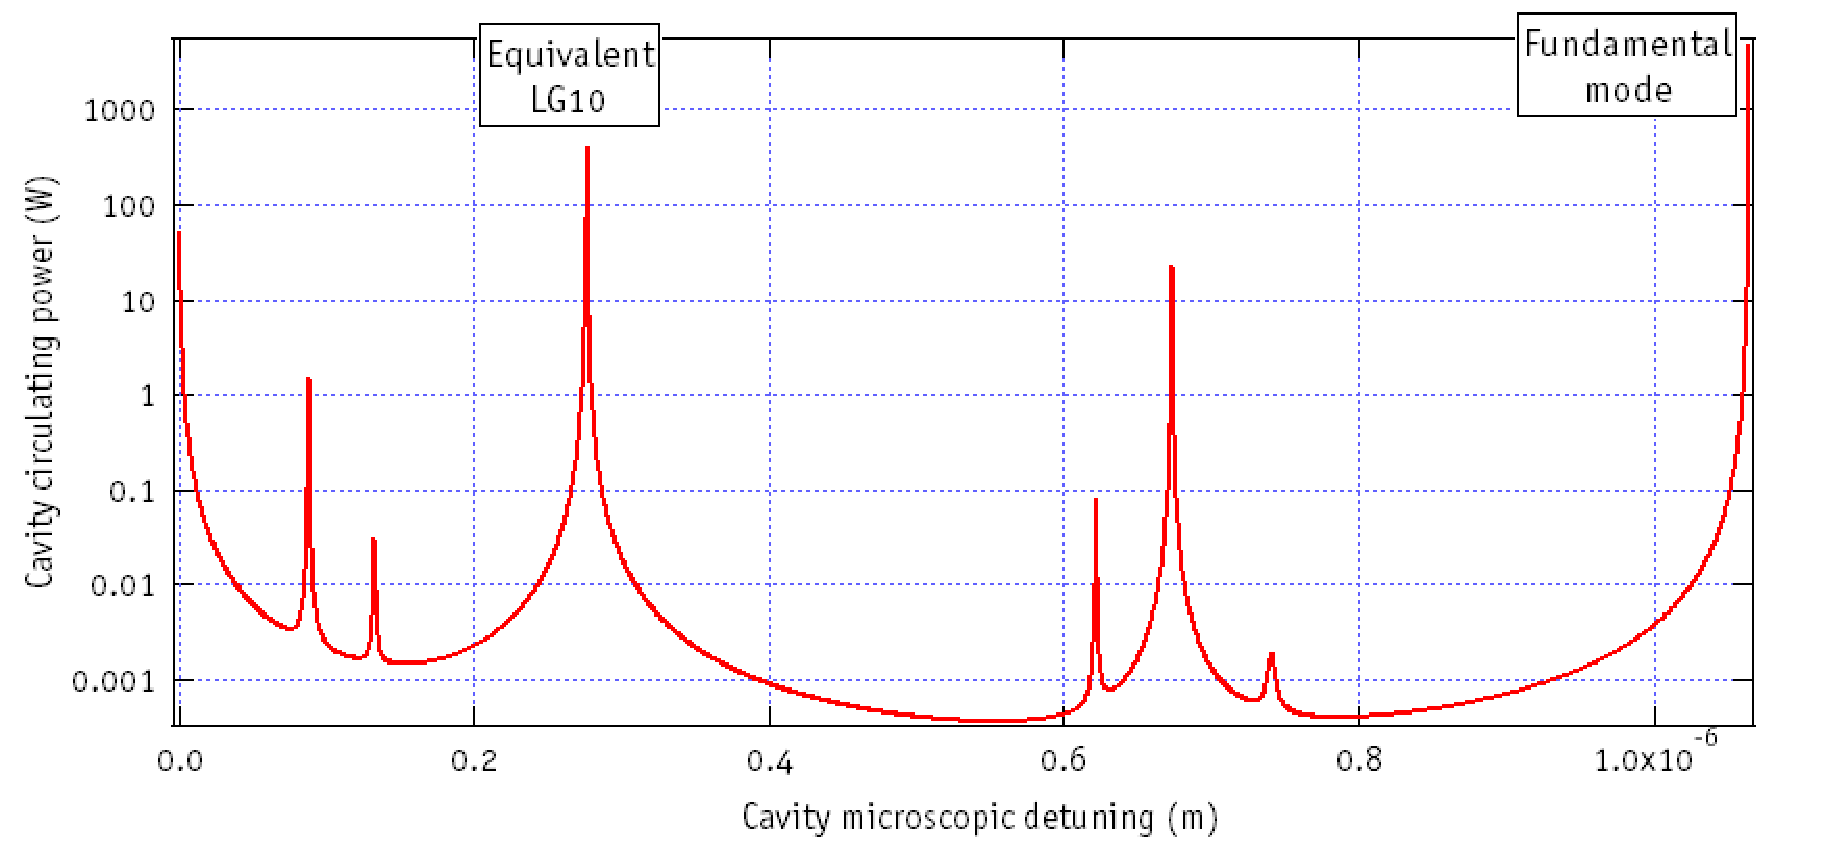
\includegraphics[width = 0.9\textwidth]{Fig3_mesa_spec.pdf}
\end{center}
\caption{Cavity spectrum of the cavity supporting flat beams. It is important to note the fundamental for a detuning of 0. This is not a coincidence, but a direct consequence of the way we defined the mirror profiles (by propagating a beam from the cavity waist).\label{fig3_mesa_spec}}
\end{figure}

Just to have a look, we can display a cross section of the fundamental flat beams and the equivalent LG$_{10}$ to compare the energy distribution. Such a comparison is shown in figure \ref{fig3_mesa_profile}.\\

\begin{figure}
\begin{center}
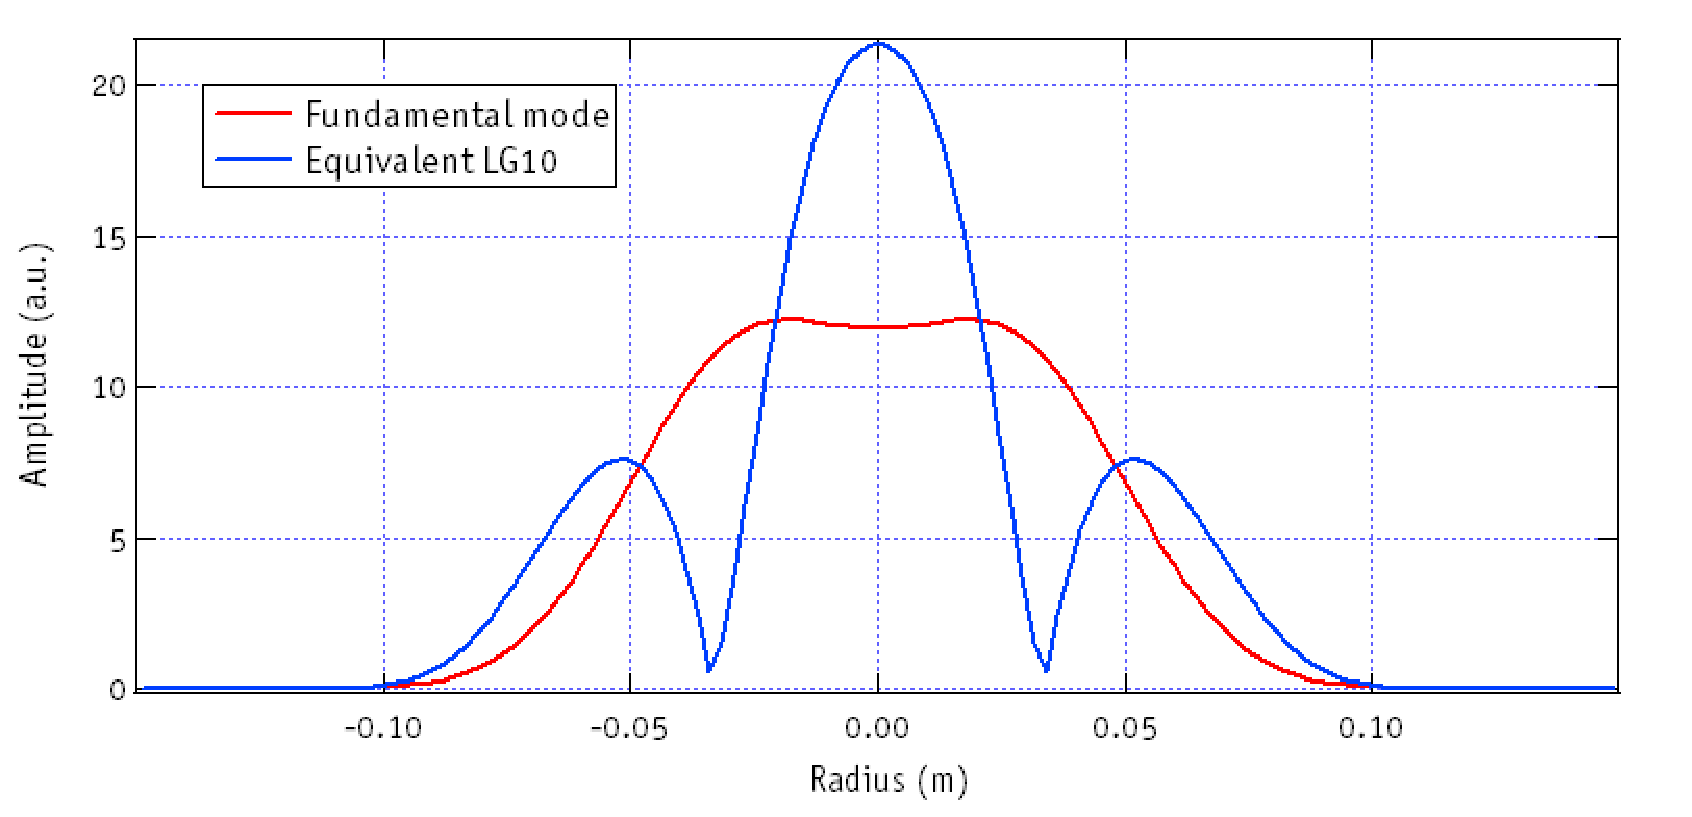
\includegraphics[width = 0.9\textwidth]{Fig3_mesa_profile.pdf}
\end{center}
\caption{Comparison of the profile of the fundamental flat beam with the equivalent LG$_{10}$. Both beam contains the same optical power.\label{fig3_mesa_profile}}
\end{figure}

So we can go back to our initial question what is the frequency separation between the fundamental mesa beam and the mode LG$_{10}$ ? From the spectrum plot, we know the difference of detuning in length between the fundamental mode and the equivalent LG$_{10}$ is $ \Delta l = 2.7664 \times 10^{-7}$~m. Since the displacement of one wavelength $\lambda$ is equivalent to one free spectral range $(c / 2L)$ , the frequency difference $\Delta f$ between the 2 modes is simply:

\begin{equation}
\begin{split}
\Delta f & = (c / 2L) * (\Delta l / \lambda)\\
& = (3 \times 10^8/4000)*( 2.7664 \times 10^{-7} / 1.064 \times 10^{-6}) \\
& = 19.5 \textrm{kHz}
\end{split}
\end{equation}

Using a similar calculation, we could also deduce the Gouy phase shift between the two cavity eigen modes.

\section{Deriving a Pound Drever Hall locking signals}
\label{cha3.4}

In this example, we will show how to implement sidebands in OSCAR. For testing purpose, we can try to derive the Pound Drever Hall (PDH) error signal which is used to lock a Fabry Perot cavity on resonance \cite{PDH}. The error signal is derived in reflection by combining a resonant (or near resonant) carrier field with a non resonant pair of sidebands. In this case, it can be shown that the error signal is in fact proportional to the imaginary part of the reflected field \cite{black:79}. The script for this example can be found in the folder \textcolor{blue}{Calculate\_PDH\_signals}

So the first thing to do, is to create sidebands using a phase modulator. Consider an electric field of amplitude $E_0$ and angular frequency $\omega_0$ incoming on a phase modulator. $E_m$ the electric field after the modulator can be written as:

\begin{equation}
\begin{split}
E_m & = E_0 \exp(i \omega_0 t + m \sin(\omega_m t))\\
    & = E_0 \exp(i \omega_0 t) \sum_{k = -\infty}^{+\infty} (-1)^k J_k(m) \exp(i k \omega_m t) \\
\end{split}
\label{eq3:bessel}
\end{equation}

\begin{table}[tbp]
  \centering
  \caption{\label{tab3:bessel} Values of the first Bessel functions for different modulating indexes m. Conveniently, the Bessel functions follow the property $J_{-k}(m) = (-1)^k J_{k}(m)$ }
\begin{tabular}{|l c c c|l|}
\hline
{\Large\strut} m & 0.1 & 0.2 & 0.4 & Taylor series\\
\hline
{\Large\strut} J$_0$(m) & 0.9975 & 0.9900 & 0.9604 & $1 - \frac{m^2}{4} + \mathcal{O}(x^4)$\\
{\Large\strut} J$_1$(m) & 0.0499 & 0.0995 & 0.1960 & $\frac{m}{2} + \mathcal{O}(x^3)$\\
{\Large\strut} J$_2$(m) & 0.0012 & 0.0050 & 0.0197 & $\frac{m^2}{8} + \mathcal{O}(x^4)$\\
{\Large\strut} J$_3$(m) & 0.0000 & 0.0002 & 0.0013 & $\frac{m^3}{48} + \mathcal{O}(x^5)$\\
\hline
\end{tabular}
\end{table}

With $m$ the modulating index and $\omega_m$ the modulation frequency. $J_k(m)$ is the bessel function of the first kind of order k. For example, the values for the first Bessel functions are shown in table \ref{tab3:bessel}. As a good approximation we can just consider the first order sidebands $k = \pm 1$. So equation \ref{eq3:bessel} can be simplified to:

\begin{equation}
E_m = E_0 \exp(i \omega_0 t) (1 + \frac{m}{2} \exp(i \omega_m t) -  \frac{m}{2} \exp(-i \omega_m t))
\end{equation}

So the electric field after the phase modulator can be expanded as the superposition of three electric fields of angular frequency $\omega_0$ (the carrier) and $\omega_0 + \omega_m$ and $\omega_0 - \omega_m$ (respectively the upper and lower sidebands). Since each field has different frequencies, they will also have different resonant conditions in the cavity.

Consider the sideband with the frequency $\omega_0 + \omega_m$. Propagating over a distance $L$ the sideband undergoes the phase shift $ \exp(i \frac{\omega_0 + \omega_m}{c} L)$. That means, the sideband phase shift is the phase shift of the carrier plus an additional phase shift. Since before entering the cavity, the carrier and the sidebands have the same spatial profile, we can simulate the sidebands in the cavity by taking the simulated carrier and by adding an extra phase shift.\\

Practically, to simulate the carrier and the sidebands, we can simulate independently three optical fields, the carrier and the lower and upper sidebands. The three fields can be treated the same way in the simulation, except that they have different round trip phase shift. Below is the three phase shifts for one round trip in the cavity:

%\begin{equation}
\begin{alignat}{2}
    \quad & \exp(i k Length.reso\_zoom) &\quad&   \text{for the carrier} \nonumber \\
    \quad & \exp(i k Length.reso\_zoom) \times \exp(i \frac{\omega_m}{c} 2 Length\_cav) && \text{for the upper sidebands} \nonumber \\
    \quad & \exp(i k Length.reso\_zoom) \times \exp(-i \frac{\omega_m}{c} 2 Length\_cav) && \text{for the lower sidebands}
\label{eq3:sid23}
\end{alignat}
%\end{equation}

As a reminder \textsl{Length\_cav} is the length of the cavity and \textsl{Length.reso\_zoom} is the microscopic tuning used to set the resonance condition for the carrier.

Since we know how to calculate the carrier and the sidebands fields circulating in the cavity, we can also calculate the reflected fields from the cavity. The reflected light is also the superposition of three fields, the reflected carrier, the reflected lower sidebands and the reflected upper sidebands with respective amplitude $E_0^{ref},\ E_-^{ref} \text{ and } E_+^{ref}$. The power $P_{det}$ detected by photodiode placed in reflection will then be:

\begin{equation}
\begin{split}
P_{det} =\ & |E_0^{ref} +  E_-^{ref}e^{-i \omega_m t} + E_+^{ref}e^{i \omega_m t}|^2 \\
     =\ & |E_0^{ref}|^2 + |E_-^{ref}|^2 + |E_+^{ref}|^2\\
    & + \cos(\omega_m t) \Re(E_0^{ref}E_-^{ref \ast}+E_0^{ref \ast}E_+^{ref})\\
    & + \sin(\omega_m t) \Im(E_0^{ref}E_-^{ref \ast}+E_0^{ref \ast}E_+^{ref})\\
    & + 2 \Re(E_+^{ref \ast}E_-^{ref} e^{-i 2\omega_m t})
\end{split}
\end{equation}

With $\Re$ and $\Im$ the real and imaginary part and $\ast$ designates the complex conjugate. The PDH error signal $e_{PDH}$ is derived by demodulating in phase $P_{det}$ and the resulting signal is then low-pass filtered. As a result $e_{PDH}$ can simply be written:

\begin{equation}
e_{PDH} = \Im(E_0^{ref}E_-^{ref \ast}+E_0^{ref \ast}E_+^{ref})
\label{A3:ePDH}
\end{equation}

The Matlab implementation of the method described above is straight forward. We first defined three electric fields: the carrier and then the lower and upper sidebands. Then we propagate each field in the cavity, calculate the reflected field and then plot the error signal using the formula \ref{A3:ePDH}. To make the result more pertinent, we fact scan the cavity over one free spectral range, so we can see the evolution of the error signal across the resonance.\\

To define the sidebands frequency and amplitude we have to define new variables (with self-explaining names) as shown in the script \ref{lis3:SB}.\\

\begin{lstlisting}[float=btp,caption=New variables to define the sidebands frequency and amplitude \label{lis3:SB},frame=lines]
% Frequency of the sidebands in Hertz and modulation index
Sidebands.frequency = 10E6;
Sidebands.modulation = 0.4;

% New carrier amplitude
Laser.amplitude = Laser.amplitude * besselj(0,Sidebands.modulation);
% Amplitude for one of the 2 sidebands
Sidebands.amplitude = besselj(1,Sidebands.modulation);
Ration_amp = Sidebands.amplitude/Laser.amplitude;

% To add the additional phase shift undergone by the sidebands during the propagation
Sidebands.k_prop = 2*pi*Sidebands.frequency/3E8;
\end{lstlisting}

Then we can calculate the three circulating fields in the cavity called \textsl{Field.Total} \textsl{Field.Total\_sidebands\_plus} and \textsl{Field.Total\_sidebands\_minus} using the usual method introduced in section \ref{sec2:4}. The only difference in the algorithm between the propagation of the carrier and the sidebands is the addition of an extra phase shift per round trip for the sidebands as shown in equation \ref{eq3:sid23}.

After we calculate the three reflected fields from the cavity named \textsl{Field.Reflect\_carrier} \textsl{Field.Reflect\_sidebands\_plus} and \textsl{Field.Reflect\_sidebands\_minus}, we can derive the PDH error signal using the formula shown by equation \ref{A3:ePDH}, the equivalent Matlab listing is shown in \ref{lis3:pdh3}.\\

\begin{lstlisting}[float=btp,caption=Calculating the PDH error signals from the fields reflected by the cavity \label{lis3:pdh3},frame=lines]
Field.PDH = imag(Field.Reflect_carrier.*conj(Field.Reflect_sidebands_plus)+...
            conj(Field.Reflect_carrier).*Field.Reflect_sidebands_minus);
% Normalised PDH signal
Power.PDH(r) = sum(sum(Field.PDH))/(Laser.amplitude*Sidebands.amplitude);
\end{lstlisting}

The plot of the power circulating in the cavity as a function of the microscopic detuning is presented in figure \ref{fig3:PDH_P}. The central peak is due to the resonance of the carrier and the two smaller peaks indicates the resonance position for the sidebands. Finally the usual PDH error signal as calculated by OSCAR is shown in figure \ref{fig3:PDH_E}. Around the resonance of the carrier, we have an error signal to lock the cavity. In theory, we have also an error signal to lock the cavity on the sidebands resonance (less useful).

\begin{figure}
\begin{center}
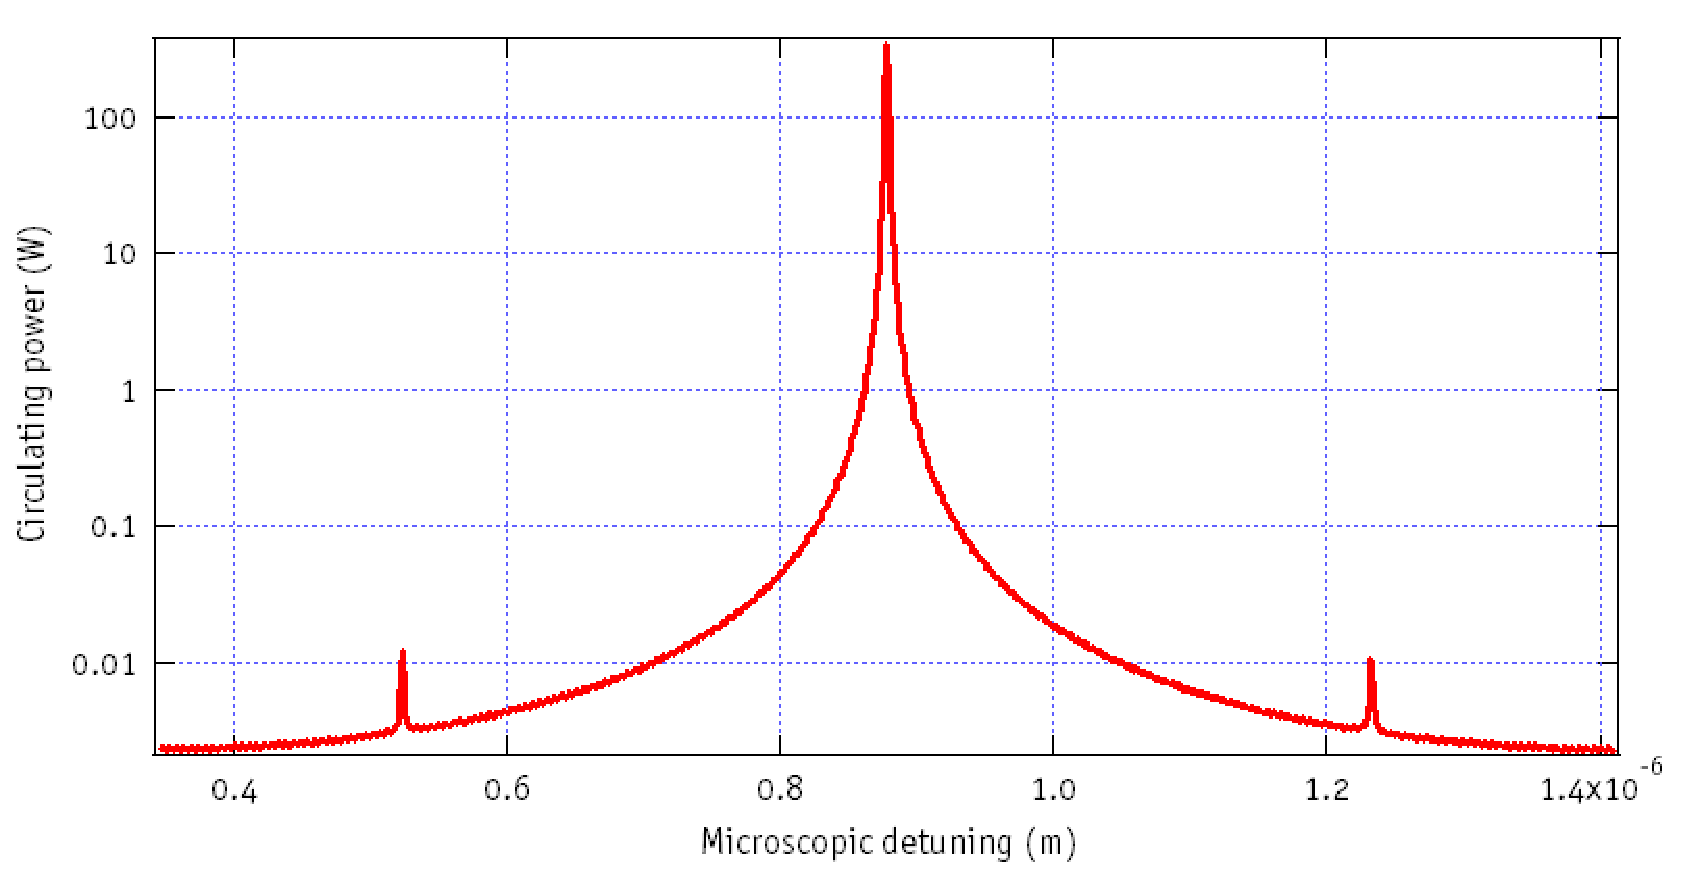
\includegraphics[width = 0.9\textwidth]{Fig3_PDH_Pcirc.pdf}
\end{center}
\caption{Circulating power inside the cavity as the cavity is scanned over one FSR. The two small peaks around the main resonance indicate the resonance of the sidebands. \label{fig3:PDH_P}}
\end{figure}

\begin{figure}
\begin{center}
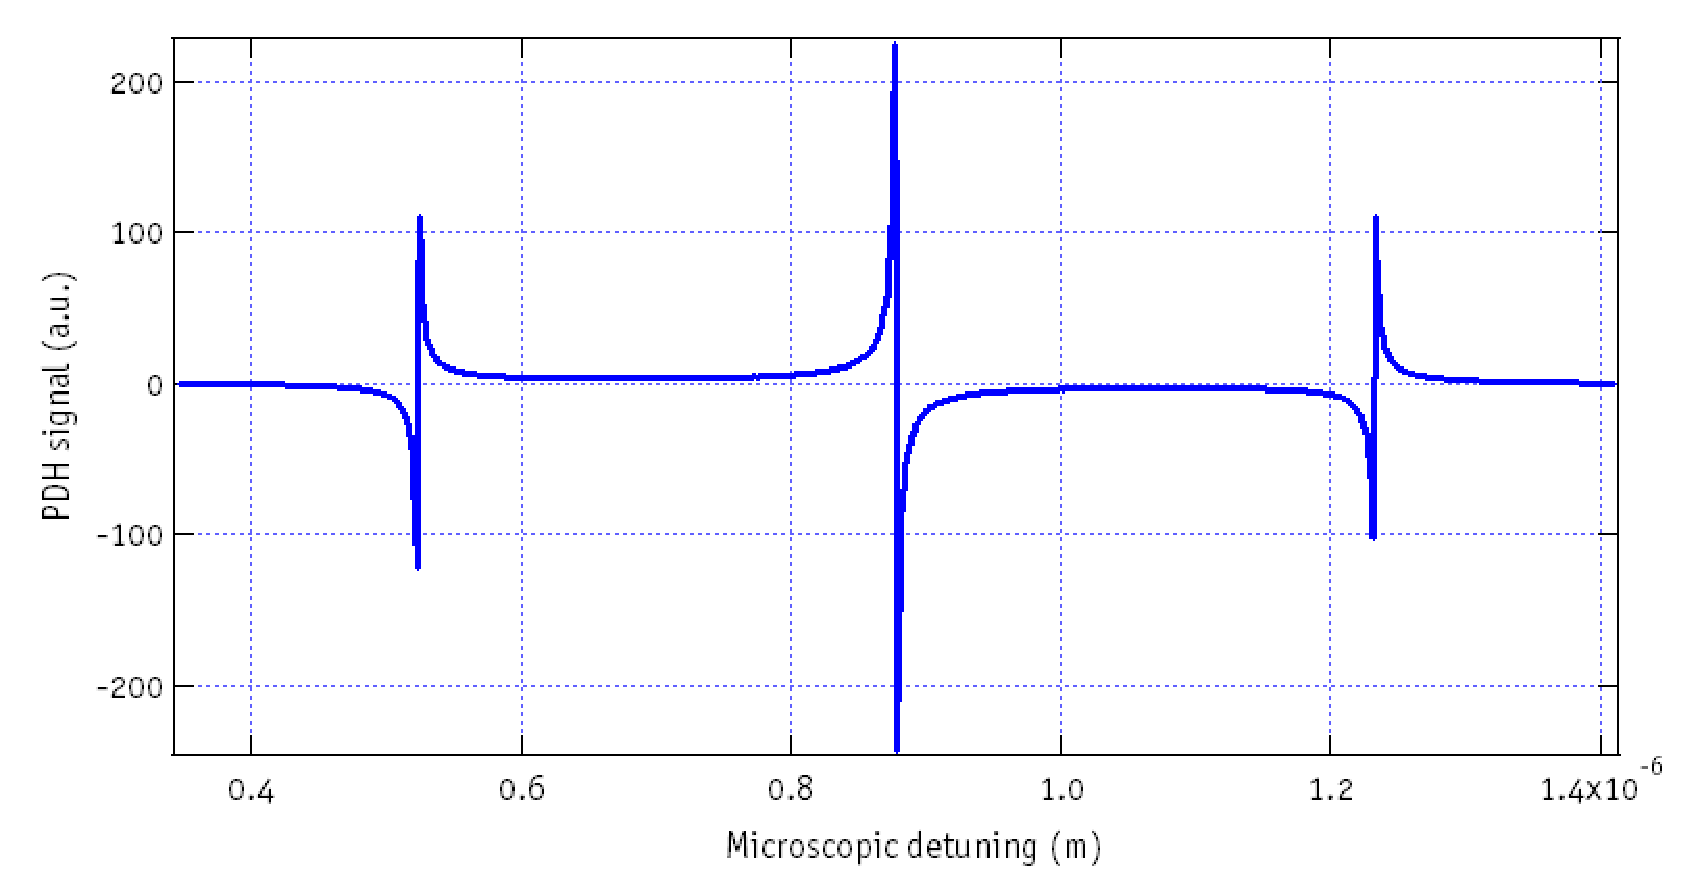
\includegraphics[width = 0.9\textwidth]{Fig3_PDH_E.pdf}
\end{center}
\caption{Pound Drever Hall error signal as a function of the detuning.\label{fig3:PDH_E}}
\end{figure}

\clearpage

\section{Simulation of a three mirrors ring cavity}
\label{cha3.5}

We can try now to add an additional mirror to our simulations and simulate a three mirrors ring cavity, often used as a mode cleaner. In the previous example we have been dealing with an optical beam perpendicular to the optical surface, this is no longer the case as seen in figure \ref{fig3:MC1}. The fact that the incident beam arrives with an angle to the surface is the main difficultly for this kind of simulation. However as we will see this problem can easily be overcome.\\

\begin{figure}
\begin{center}
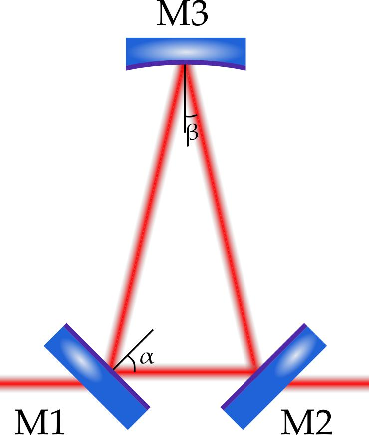
\includegraphics[width = 0.5\textwidth]{Fig3_MC.pdf}
\end{center}
\caption{Optical setup of a three mirrors ring cavity. Unlike a Fabry-Perot cavity, where the mirrors are usually perpendicular to the incident beam, for the mode cleaner the incoming beam arrives with a large angle on the two bottom mirrors. The mirror notation used in the OSCAR example are also indicated. \label{fig3:MC1}}
\end{figure}

In the OSCAR mode cleaner example (folder \textcolor{blue}{Simulate\_mode\_cleaner}), we suppose that the incident plane is horizontal. We keep this convention in the manual and it is relatively easy to adapt the code for any arbitrary angle of incidence. Let's examine what is happening on reflection: as soon as the angle of incidence of an electric field to a reflective surface is different from zero, two effects can arise:
\begin{itemize}
  \item The reflected beam will present astigmatism directly related to the angle of incidence.
  That can be understood by imagining that the incident beam will be stretched in the horizontal direction as it is projected to the mirror surface upon reflection.
  \item The beam on reflection will get flipped in the horizontal direction, this is purely a geometrical effect and the reader can easily be convinced by looking at the figure \ref{fig3:MC_flip}.
\end{itemize}

\begin{figure}
\begin{center}
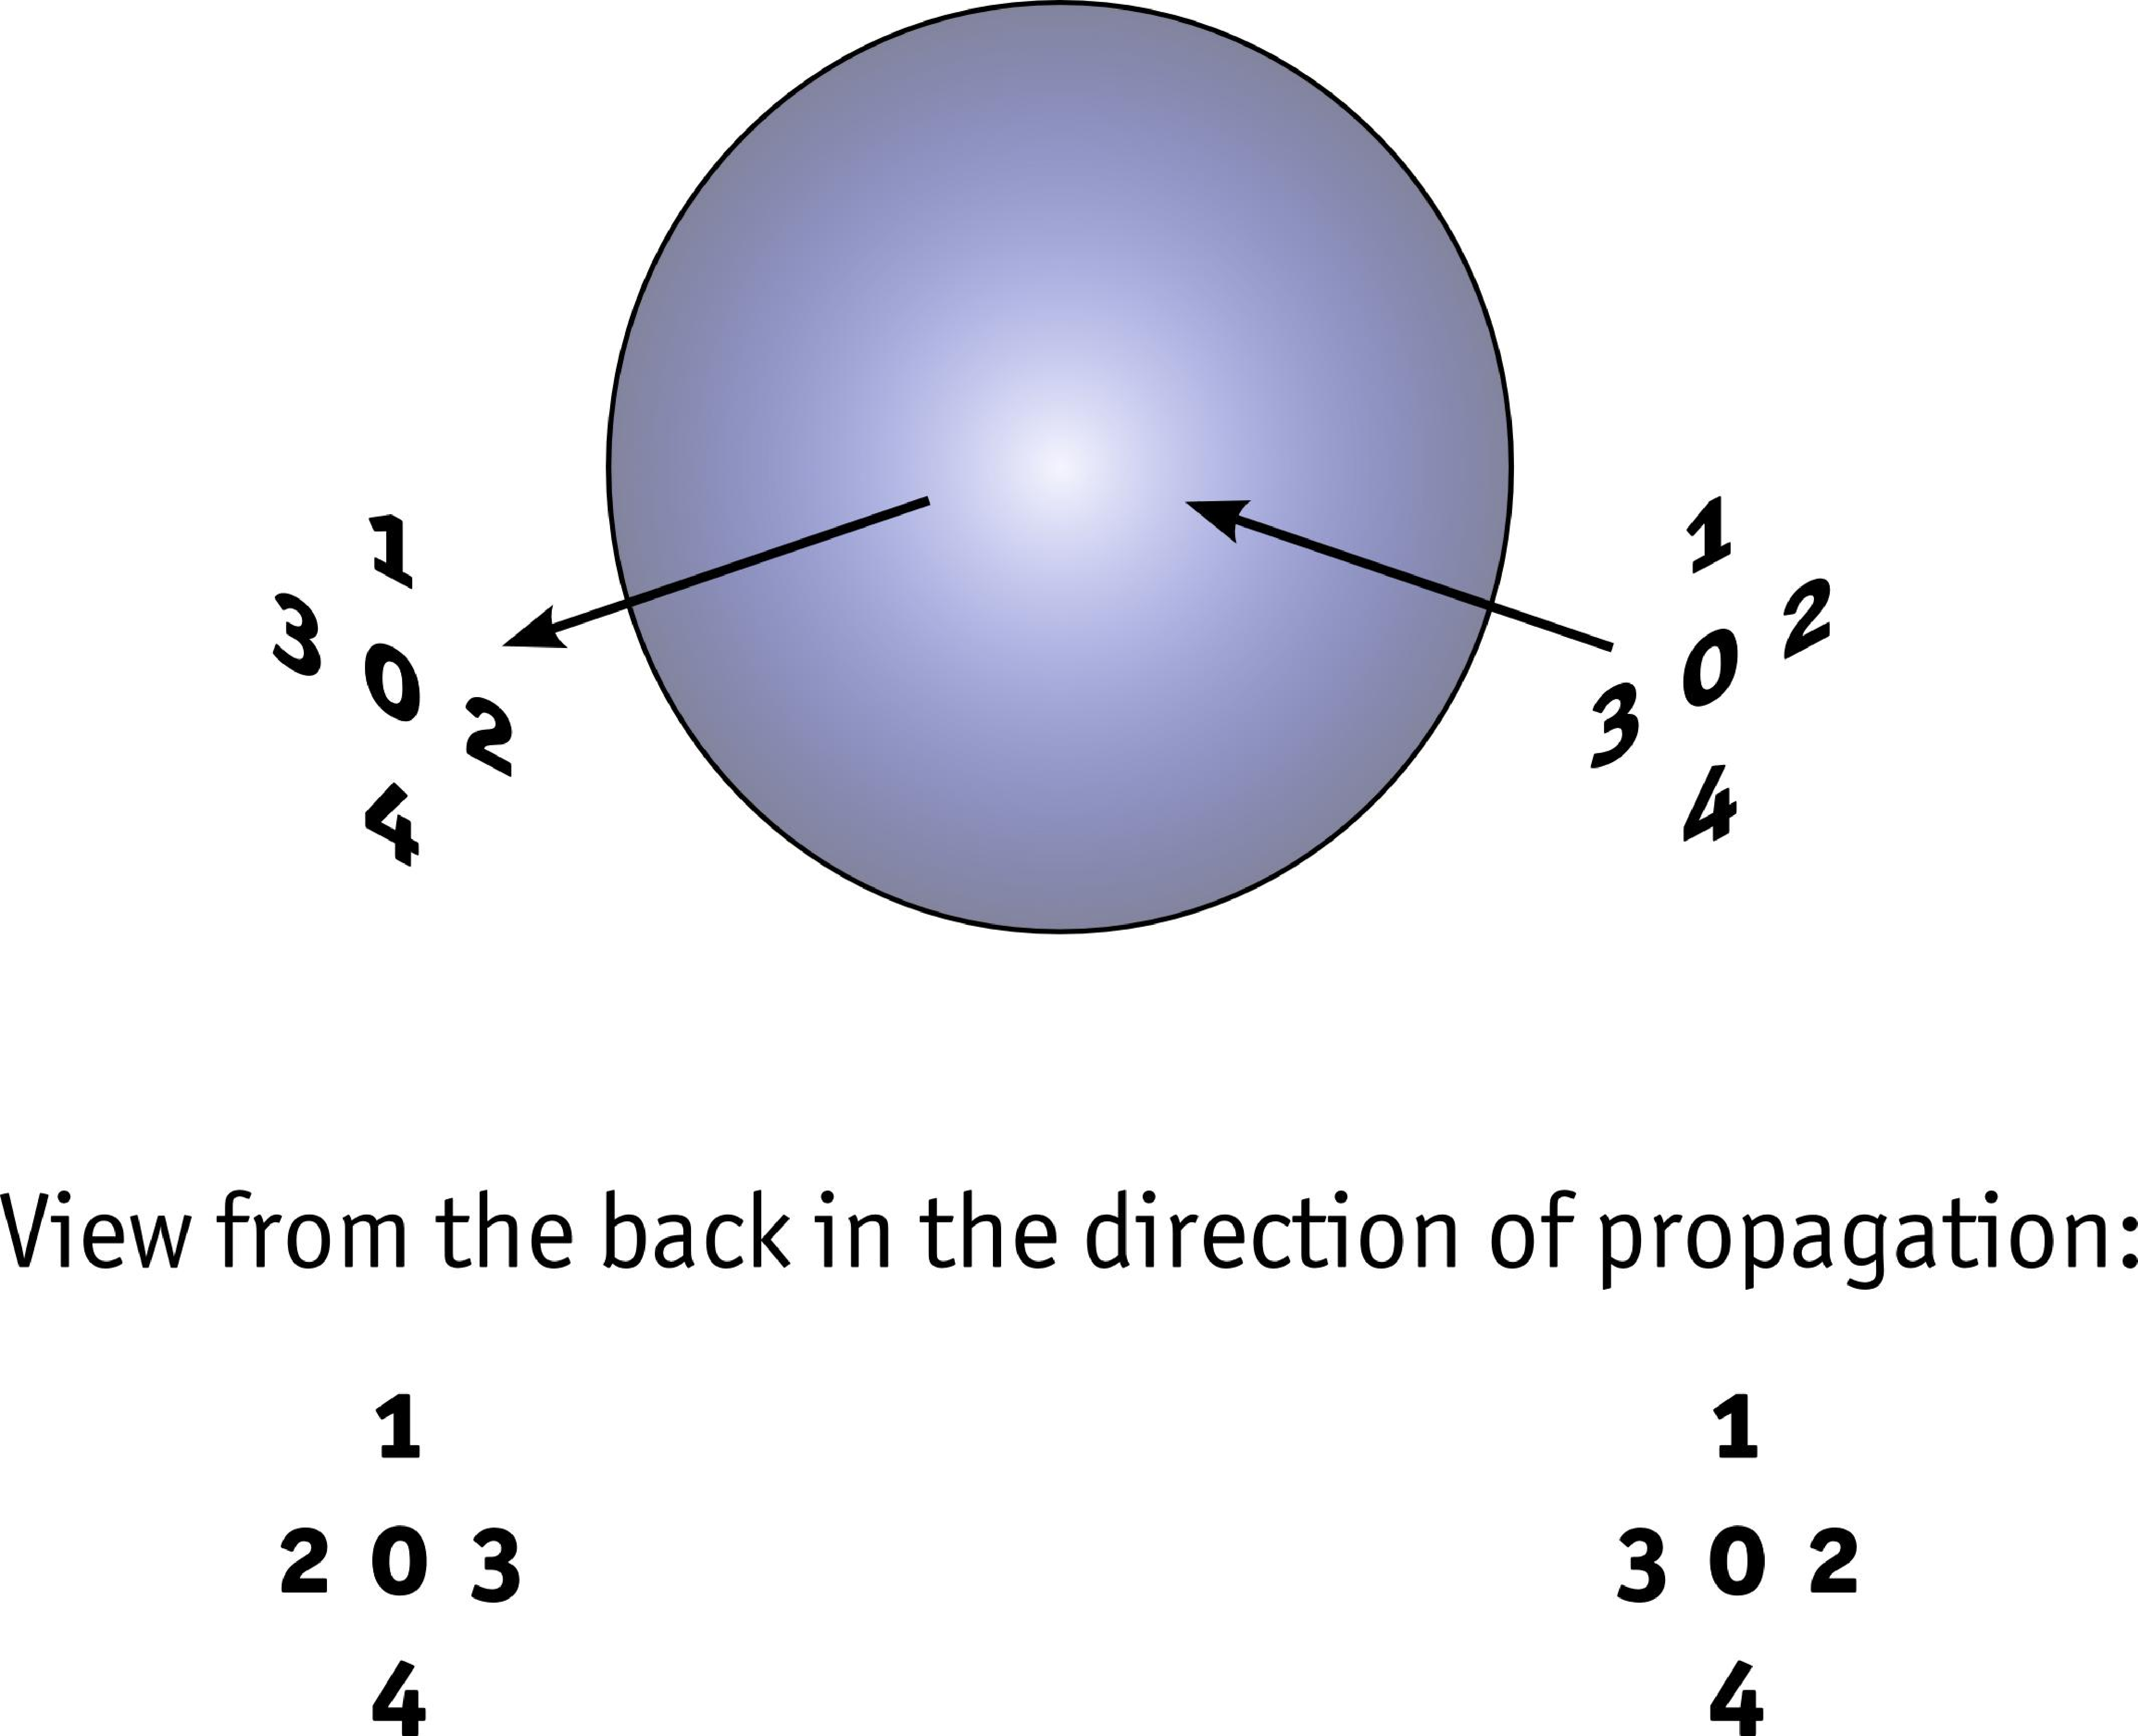
\includegraphics[width = 0.5\textwidth]{Fig3_MC_flip.pdf}
\end{center}
\caption{Example of an image reflected by a mirror. It is interesting to see that after reflection the image is flipped in the horizontal direction. \label{fig3:MC_flip}}
\end{figure}

The two items described above are implemented in OSCAR in the new function \emph{Propa\_mirror} showed in the listing \ref{lis3:mc}. Compared to the function \emph{Propa\_mirror} seen in the first chapter (section \ref{sec1:3:5}), we have added one new input parameter: \textsl{Grid\_angle\_X}. \textsl{Grid\_angle\_X} is a new distorted 2D grid representing the projection of the grid used for propagation (called \textsl{Grid.D2}) to the mirror surface.

\begin{lstlisting}[float=btp,caption=Reflection on a mirror for arbitrary angle of incidence\label{lis3:mc},frame=lines]
% Stretch the laser beam as seen by the mirror
Output = Propa_mirror(Wave_field, Wave_mirror, reflec,Grid_angle_X)

Output = interp2(Grid_angle_X,Grid.Y,Wave_field,Grid.X,Grid.Y,'cubic');

Output = Output .* exp(-i * Wave_mirror*Laser.k_prop) * reflec .* Mirror.mask;


% Go back to the normal grid
Output = interp2(Grid.X,Grid.Y,Output,Grid_angle_X,Grid.Y,'cubic',0);

% Flip the matrix along the x axis
Output = Output(:,Grid.Num_point:-1:1);
\end{lstlisting}

The function used to simulate the reflection on a mirror can be decomposed in the following steps:
\begin{enumerate}
  \item Project the incident beam on the mirror surface. So the incident beam will look astigmatic.
  \item Reflect the projected incident beam in the same way as a incoming beam normal to the mirror surface
  \item Project the reflected beam to the on the plane of propagation
  \item Flip the beam in the horizontal plane
\end{enumerate}

The steps described above are directly implemented in Matlab as shown in the script \ref{lis3:mc}.

In the examples provided with OSCAR, the transmission of a 3 mirrors ring cavity is presented. To show the mode cleaning effect, the input beam is the normalised sum of the TEM$_{10}$ and TEM$_{01}$. As expected both modes have different resonance condition inside the mode cleaner as shown in figure \ref{fig3:MC_reso}. The microscopic resonance length of the two modes is separated by half a wavelength, which is the expected result since the mode TEM$_{10}$ encountered an extra $3\pi$ shift during its round trip propagation.


\begin{figure}
\begin{center}
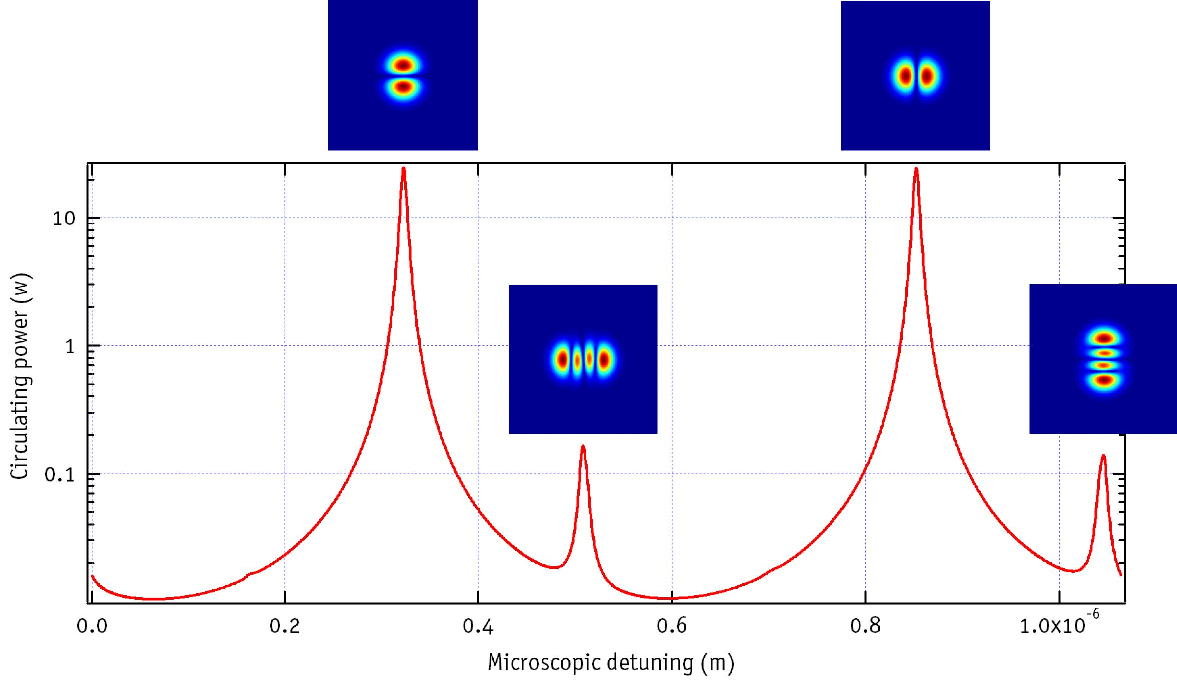
\includegraphics[width = 0.8\textwidth]{Fig3_MC_reso.pdf}
\end{center}
\caption{Scan of the mode cleaner over one free spectral range. The two main peaks are due to the resonance of the TEM$_{01}$ and TEM$_{10}$. Additional peaks in the spectrum indicates a slight modemismatching. \label{fig3:MC_reso}}
\end{figure}


For this example, we set the working point of the cavity for the mode TEM$_{10}$ to be resonant inside the cavity. The transmitted field from the mode cleaner is shown at the bottom right corner of figure \ref{fig3:MC_res}. As we would hope the transmitted field is a pure TEM$_{10}$. For consistency, we also check that the reflected field is very similar to a pure TEM$_{01}$, but not exactly since the input beam was not perfectly matched to the cavity.

\begin{figure}
\begin{center}
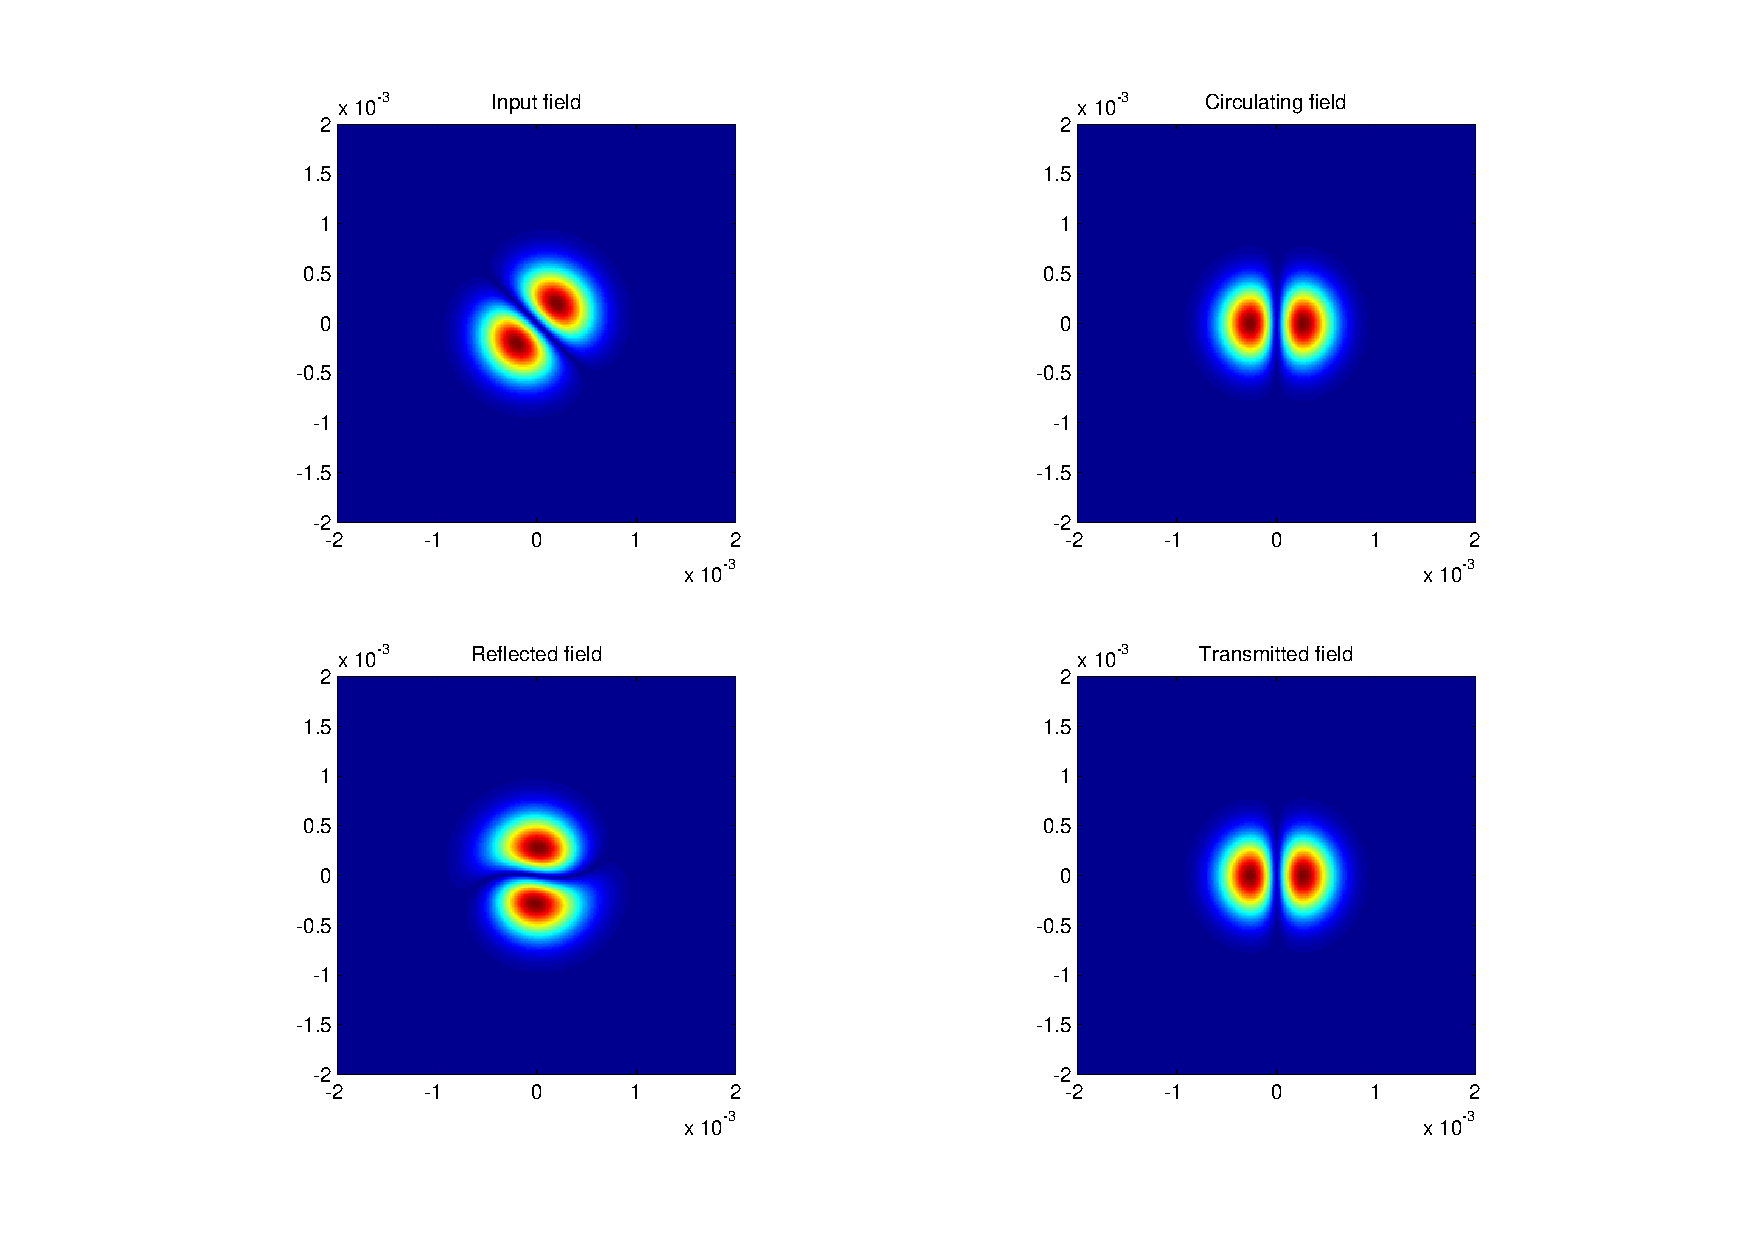
\includegraphics[width = 1.0\textwidth]{Fig3_MC_res2.pdf}
\end{center}
\caption{Output screen from OSCAR. The input field, a sum of TEM$_{10}$ and TEM$_{01}$ is shown on the top left corner. The reflected and the transmitted field are shown respectively in the bottom left and right picture.  \label{fig3:MC_res}}
\end{figure}

Below is the output from OSCAR:

\begin{verbatim}
 ------ Display the results ------
 Circulating power (W): 49.524735
 Reflected power (W): 0.503506
 Transmitted power (W): 0.495243
\end{verbatim}

So the mode cleaner was able to separate the mode TEM$_{10}$ and TEM$_{01}$. We have slightly more power reflected than transmitted by the cavity, this is a direct consequence of the fact that the input beam is not perfectly matched to the cavity.

\begin{verbatim}
 ---- Display results for cavity C1 -----
 Round trip diffraction loss: 35.6127 [ppm]
 Circulating power: 49.8224 [W]
 Size of the beam on the end mirror: 0.0205821 [m]
 Size of the beam on the input mirror: 0.020576 [m]
 Size of the cavity waist: 0.0183982 [m]
 Distance of the cavity waist from the input mirror: -500.471 [m]
\end{verbatim}


